%!TEX root = ../username.tex
\lstset{
    backgroundcolor=\color{white},
    basicstyle=\footnotesize\ttfamily,
    breaklines=true,
    frame=single,
    captionpos=b,
    numbers=left,
    numberstyle=\tiny\color{gray},
    keywordstyle=\color{blue},
    commentstyle=\color{green},
    stringstyle=\color{red}
}
\chapter{Architecture of My Digital Wardrobe}
\label{chap:Chapter4}

{Integration of Different System Architecture}
In this Chapter we will discuss the different Architectures that work together to develop this application. 
 The architecture of \textit{My Digital Wardrobe} combines two key systems:\textbf{Client-Server} and \textbf{React Native Architecture}. These systems work together to create a mobile application that allows users to easily manage their wardrobes, upload images, and create outfit combinations. The frontend allows users to interact with the app smoothly, while Firebase manages data storage, authentication, and images. This setup lets users access their wardrobe from any device.
 

\section{The Client-Server Architecture}

The \textbf{Client-Server Architecture } 
describes how two main parts of the application—the \textbf{client} and the \textbf{server} —communicate with each other to make the app function smoothly.

\noindent \textbf{Understanding the Client and Server Roles}:
\begin{itemize}
    \item \textbf{Client (Frontend)}: The client is the part of the app that users see and interact with on their mobile devices. In My Digital Wardrobe, the client is built using React Native and Expo, which means the app looks and feels like a native mobile app on both iOS and Android. When users perform actions such as uploading a clothing image, browsing wardrobe items, or creating an outfit, the client sends these requests to the server.
    \item \textbf{Server (Backend)}: The server is like the "brain" behind the app, handling data processing and storage. In this app, Firebase acts as the server. It manages tasks such as storing user-uploaded images, saving wardrobe information, and authenticating users during login. Firebase also ensures that users’ data is securely stored and accessible only to them.
    
\end{itemize}

\noindent \textbf{How the Client and Server Work Together}:

When a user uploads a picture of a clothing item, the client (app on the phone) sends this image to Firebase (server). Firebase stores the image and sends back a confirmation that the upload was successful. The app then displays this image in the user’s wardrobe. This process happens in real-time, meaning that as soon as the server processes the data, the client updates the user interface accordingly.

This interaction allows the app to perform complex tasks like image storage and data management without slowing down the user’s phone. The heavy processing is done on Firebase’s servers, while the user enjoys a fast and responsive experience on their device.

\begin{figure}[h]
    \centering
    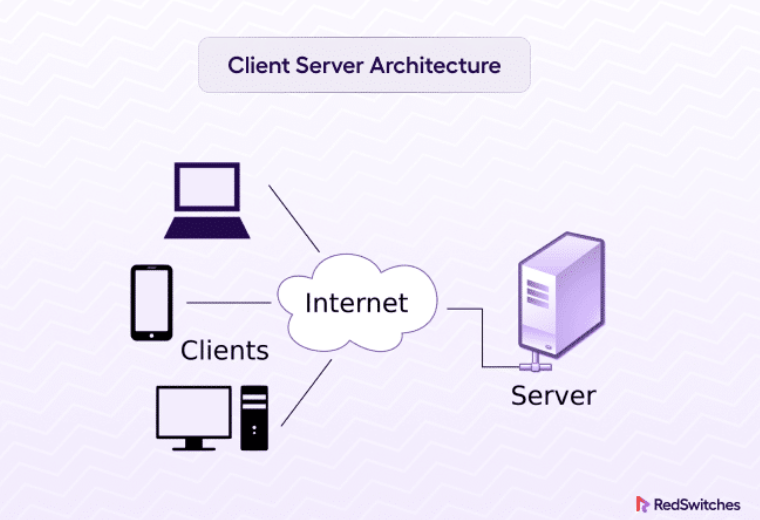
\includegraphics[width=0.9\linewidth]{exampleis-master/figures/C-S.png}
    \caption{The Client-Server architecture \cite{client_server_arch}}
    \label{fig:client_server_architecture}
\end{figure}

In Figure \ref{fig:client_server_architecture}, we can see that the client and server communicate continuously.
This client-server relationship ensures that the app remains lightweight on the client side while utilizing Firebase’s robust backend services for heavy-lifting operations such as storage and authentication\cite{client_server_arch}.

\section{React Native + Expo Architecture}

The frontend utilizes the \textbf{React Native + Expo Architecture}, enabling cross-platform compatibility while consisting  a modular and maintainable codebase. In simple terms, this architecture allows the app to work smoothly on both iOS and Android devices without the need to create two separate versions.
\textbf{React Native}, as discussed in the previous chapter(Chapter \ref{chap:Chaptert3}), enables the development of mobile applications using a single codebase across differnet devices. This ensures consistency across platforms while reducing development time and effort.

\textbf{Expo} complements React Native by providing tools and libraries that streamline common development tasks. It simplifies access to device-specific features such as the camera, image gallery, and navigation, eliminating the need for additional native code and accelerating the development process.

As seen in Figure \ref{fig:react_native_architecture} React Native's architecture revolves around the \textbf{Bridge Model}, which facilitates communication between the JavaScript logic and the Native components of the app \cite{react_native_arch}. Expo further enhances this framework by providing pre-built libraries and access to device-specific features, streamlining the development and deployment process.


\noindent \textbf{The main three features of React Native + Expo Architecture are }:
\begin{enumerate}
    \item \textbf{Declarative UI Design}: React Native allows us to describe what the app should look like, and it automatically updates the screen when the app’s data changes. This makes the user experience smoother, as the app responds immediately to user actions.
    \item \textbf{Cross-Platform Compatibility}: The architecture ensures that the app works the same way different devices without having to build two separate apps.
    \item \textbf{Expo's Prebuilt Libraries}: Expo simplifies development by offering APIs for native functionalities such as the camera, image picker, and navigation, eliminating the need for custom native modules in most scenarios.
\end{enumerate}
Next, we explain how the components in the Figure \ref{fig:react_native_architecture} work together in our app.
The React Native + Expo Architecture relies on a layered structure where each part has a specific job:
\begin{enumerate}

    \item\textbf{React Layer (User Interface and Logic)}:
This is the layer where developers write the code that defines how the app looks and behaves. For example, when users browse their wardrobe or select outfits, this layer controls what they see on the screen and how they interact with it.

    \item \textbf{JavaScript Thread (The Brain of the App)}:
This layer runs the JavaScript code that powers the app’s logic. It manages user interactions, such as tapping buttons or selecting images, and decides what should happen next.

    \item \textbf{Bridge Layer (The Translator)}:
The Bridge acts as a translator between the JavaScript code and the device’s native features. Since mobile devices run on native code, the bridge ensures that commands written in JavaScript are correctly understood by the phone’s operating system. For instance, when a user selects an image to upload, the bridge translates this action so the phone can access the image from the gallery.

    \item \textbf{Native Layer (Device-Specific Features)}:
This is where the app connects with the device’s built-in functions, such as the camera, storage, or touch gestures. It ensures that animations run smoothly, images load quickly, and user interactions feel natural and responsive.
\end{enumerate}


\begin{figure}[h]
    \centering
    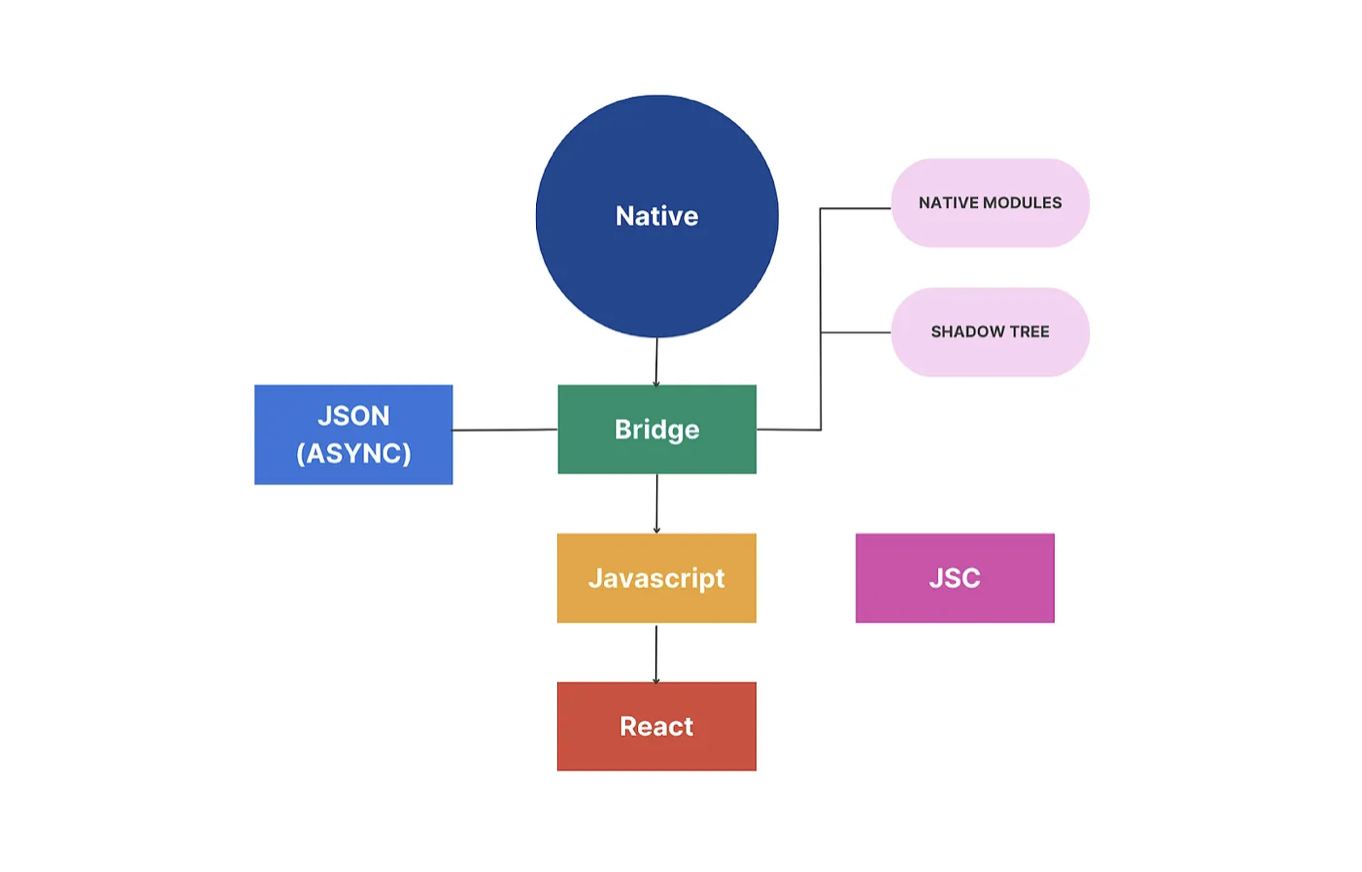
\includegraphics[width=0.8\linewidth]{exampleis-master/figures/ReactNative.png}
    \caption{The React Native  architecture \cite{react_native_arch} }
    \label{fig:react_native_architecture}
\end{figure}


Next, to better understand how this architecture functions, lets consider the process of a user uploading an image of a clothing item in \textbf{ My Digital Wardrobe}:

\begin{itemize}
    \item \textbf{Step 1: User Action }A user uploads an image.
    \item \textbf{Step 2: React Layer Response }The React layer triggers Expo’s ImagePicker API, which opens the device’s gallery.
    \item \textbf{Step 3: Bridge in Action }The bridge translates this request from JavaScript into a command the phone understands, allowing access to the gallery.
    \item \textbf{Step 4: Native Layer Processing }The user selects an image, and the native layer retrieves it from the phone’s storage.
    \item \textbf{Step 5: Data Sent Back }The image is sent back through the bridge to the JavaScript layer for further processing such as resizing or preview rendering can occur.
    \item \textbf{Step 6: Storage in Firebase }Finally, the image is uploaded to Firebase, where it is stored securely and displayed in the user’s digital wardrobe ready for viewing, editing, or mixing and matching with other clothing items.
    
\end{itemize}


This architecture ensures that the app benefits from React Native's flexibility for building responsive, modular components while utilizing Expo's tools to handle platform-specific integrations. By utilizing the Bridge model, \textit{My Digital Wardrobe} achieves a balance between cross-platform efficiency and near-native performance.

\section{Backend and Data Storage}

Firebase serves as the \textit{Backend-as-a-Service (BaaS)} for \textit{My Digital Wardrobe}, streamlining backend management and providing powerful features such as \textbf{real-time data synchronization}, \textbf{secure cloud storage}, and \textbf{user authentication}. This architecture eliminates the need for dedicated servers, allowing the app to directly interact with Firebase services via its SDKs, ensuring scalability and ease of integration \cite{firebase_intro}.

\begin{figure}[h]
    \centering
    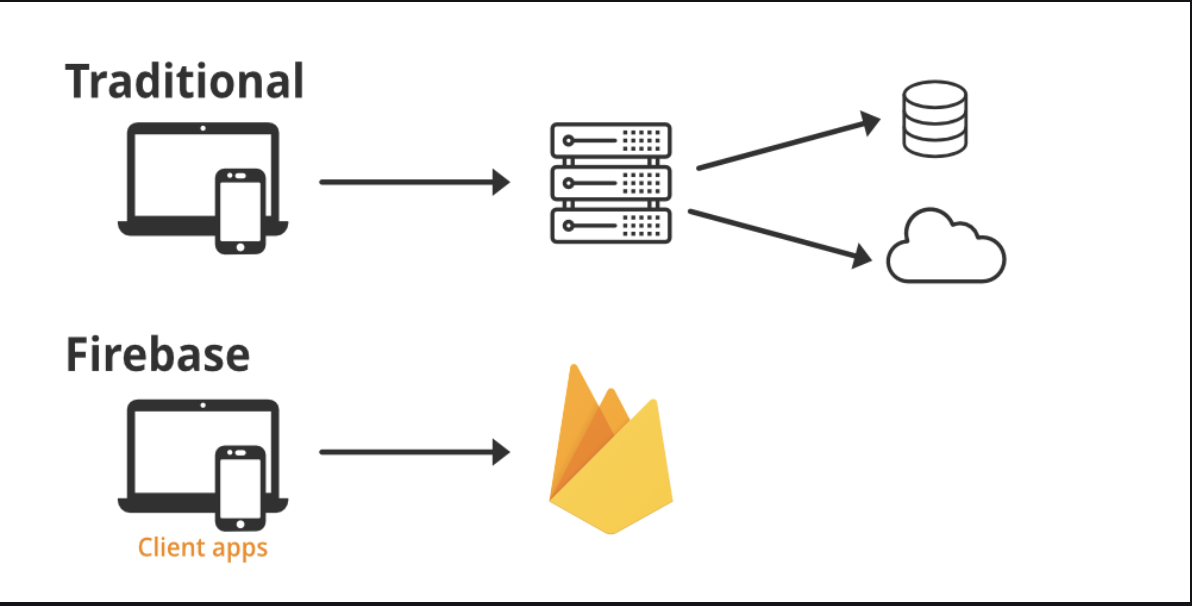
\includegraphics[width=0.6\linewidth]{exampleis-master/figures/firebase.png}
    \caption{Firebase as a Backend-as-a-Service\cite{firebase_intro}}
    \label{fig:firebase_backend}
\end{figure}

\subsection{Traditional Databases vs. Firebase (Firestore)}

To understand why Firebase is ideal for My Digital Wardrobe, it’s helpful to compare it with a traditional database.
\begin{itemize}
    \item \textbf{Traditional Databases:}
These databases, such as\textbf{ MySQL} or \textbf{PostgreSQL}, store data in tables with rows and columns, similar to a spreadsheet. To access or update data, applications typically need a separate server that handles communication between the app and the database (see Figure \ref{fig:firebase_backend}. For example, when a user uploads an image, the request first goes to the server, which then stores the image in the database and sends a response back. While this approach is reliable, it can be slower and more complex, especially when handling real-time updates across multiple users.

\item \textbf{Firebase Firestore (NoSQL Database):}
In contrast, Firestore—the database used by Firebase—stores data in a more flexible structure using collections and documents, similar to a filing cabinet with labeled folders. For My Digital Wardrobe, one collection might store wardrobe items, while another stores outfit combinations. Each document in a collection contains key-value pairs, making it easy to store diverse data like image URLs, categories, and timestamps.
Unlike traditional databases, Firestore allows the app to communicate directly with the database, eliminating the need for a separate server. This direct connection ensures real-time synchronization, meaning any changes users make (like uploading a new clothing item) are instantly visible in the app without refreshing or waiting.
\end{itemize}
\subsection{Firebase in My Digital Wardrobe}
In this section, we discuss how \textbf{Firebase} provides two core services that are essential for managing wardrobe data and images:
\begin{enumerate}
    \item \textbf{Cloude Storage for Images}
    When users upload photos of clothing items, these images are stored in Firebase Cloud Storage. Each image is given a unique web link (URL), allowing the app to retrieve and display it whenever needed. This process happens in the background, ensuring that images load quickly without slowing down the app.
    \item \textbf{Firestore Database for Organizing Wardrobe Items}
    The Firestore database organizes all user data related to clothing items and outfits. It keeps everything neatly structured, making it easy for users to browse, sort, and filter their wardrobe. Key information stored in Firestore includes:
   
    \begin{itemize}
        \item \textbf{Categories}: Classifications like tops, bottoms,  enabling easy filtering and browsing within the app.
        \item \textbf{File Names}: Unique identifiers for each uploaded image, generated with timestamps and random identifiers to ensure no file overwriting occurs.
        \item \textbf{Image URLs}: Direct links to the images stored in Firebase Cloud Storage, used to retrieve and display the images in the app’s interface.
        \item \textbf{Timestamps}: Date and time of upload, which can be used to organize and sort wardrobe items chronologically.
    \end{itemize}
\end{enumerate}


The Firestore database serves as the backbone for data management in the application. As illustrated in Figure \ref{fig:firestore_collections}, the database structure is designed to support two key functionalities: managing individual wardrobe items and storing outfit combinations. 
\begin{enumerate}
    \item \textbf{Wardrobe Items:} Storing individual clothing pieces with relevant details like category and image location.
    \item \textbf{Outfit Items:} Saving user-created outfits by linking selected wardrobe items together, allowing users to revisit and reuse their favorite combinations.
\end{enumerate}

\begin{figure}[!ht]\centering
    % First Subfloat: Wardrobe Items
    \subfloat[Firestore structure for wardrobe items.][Wardrobe Items]
    {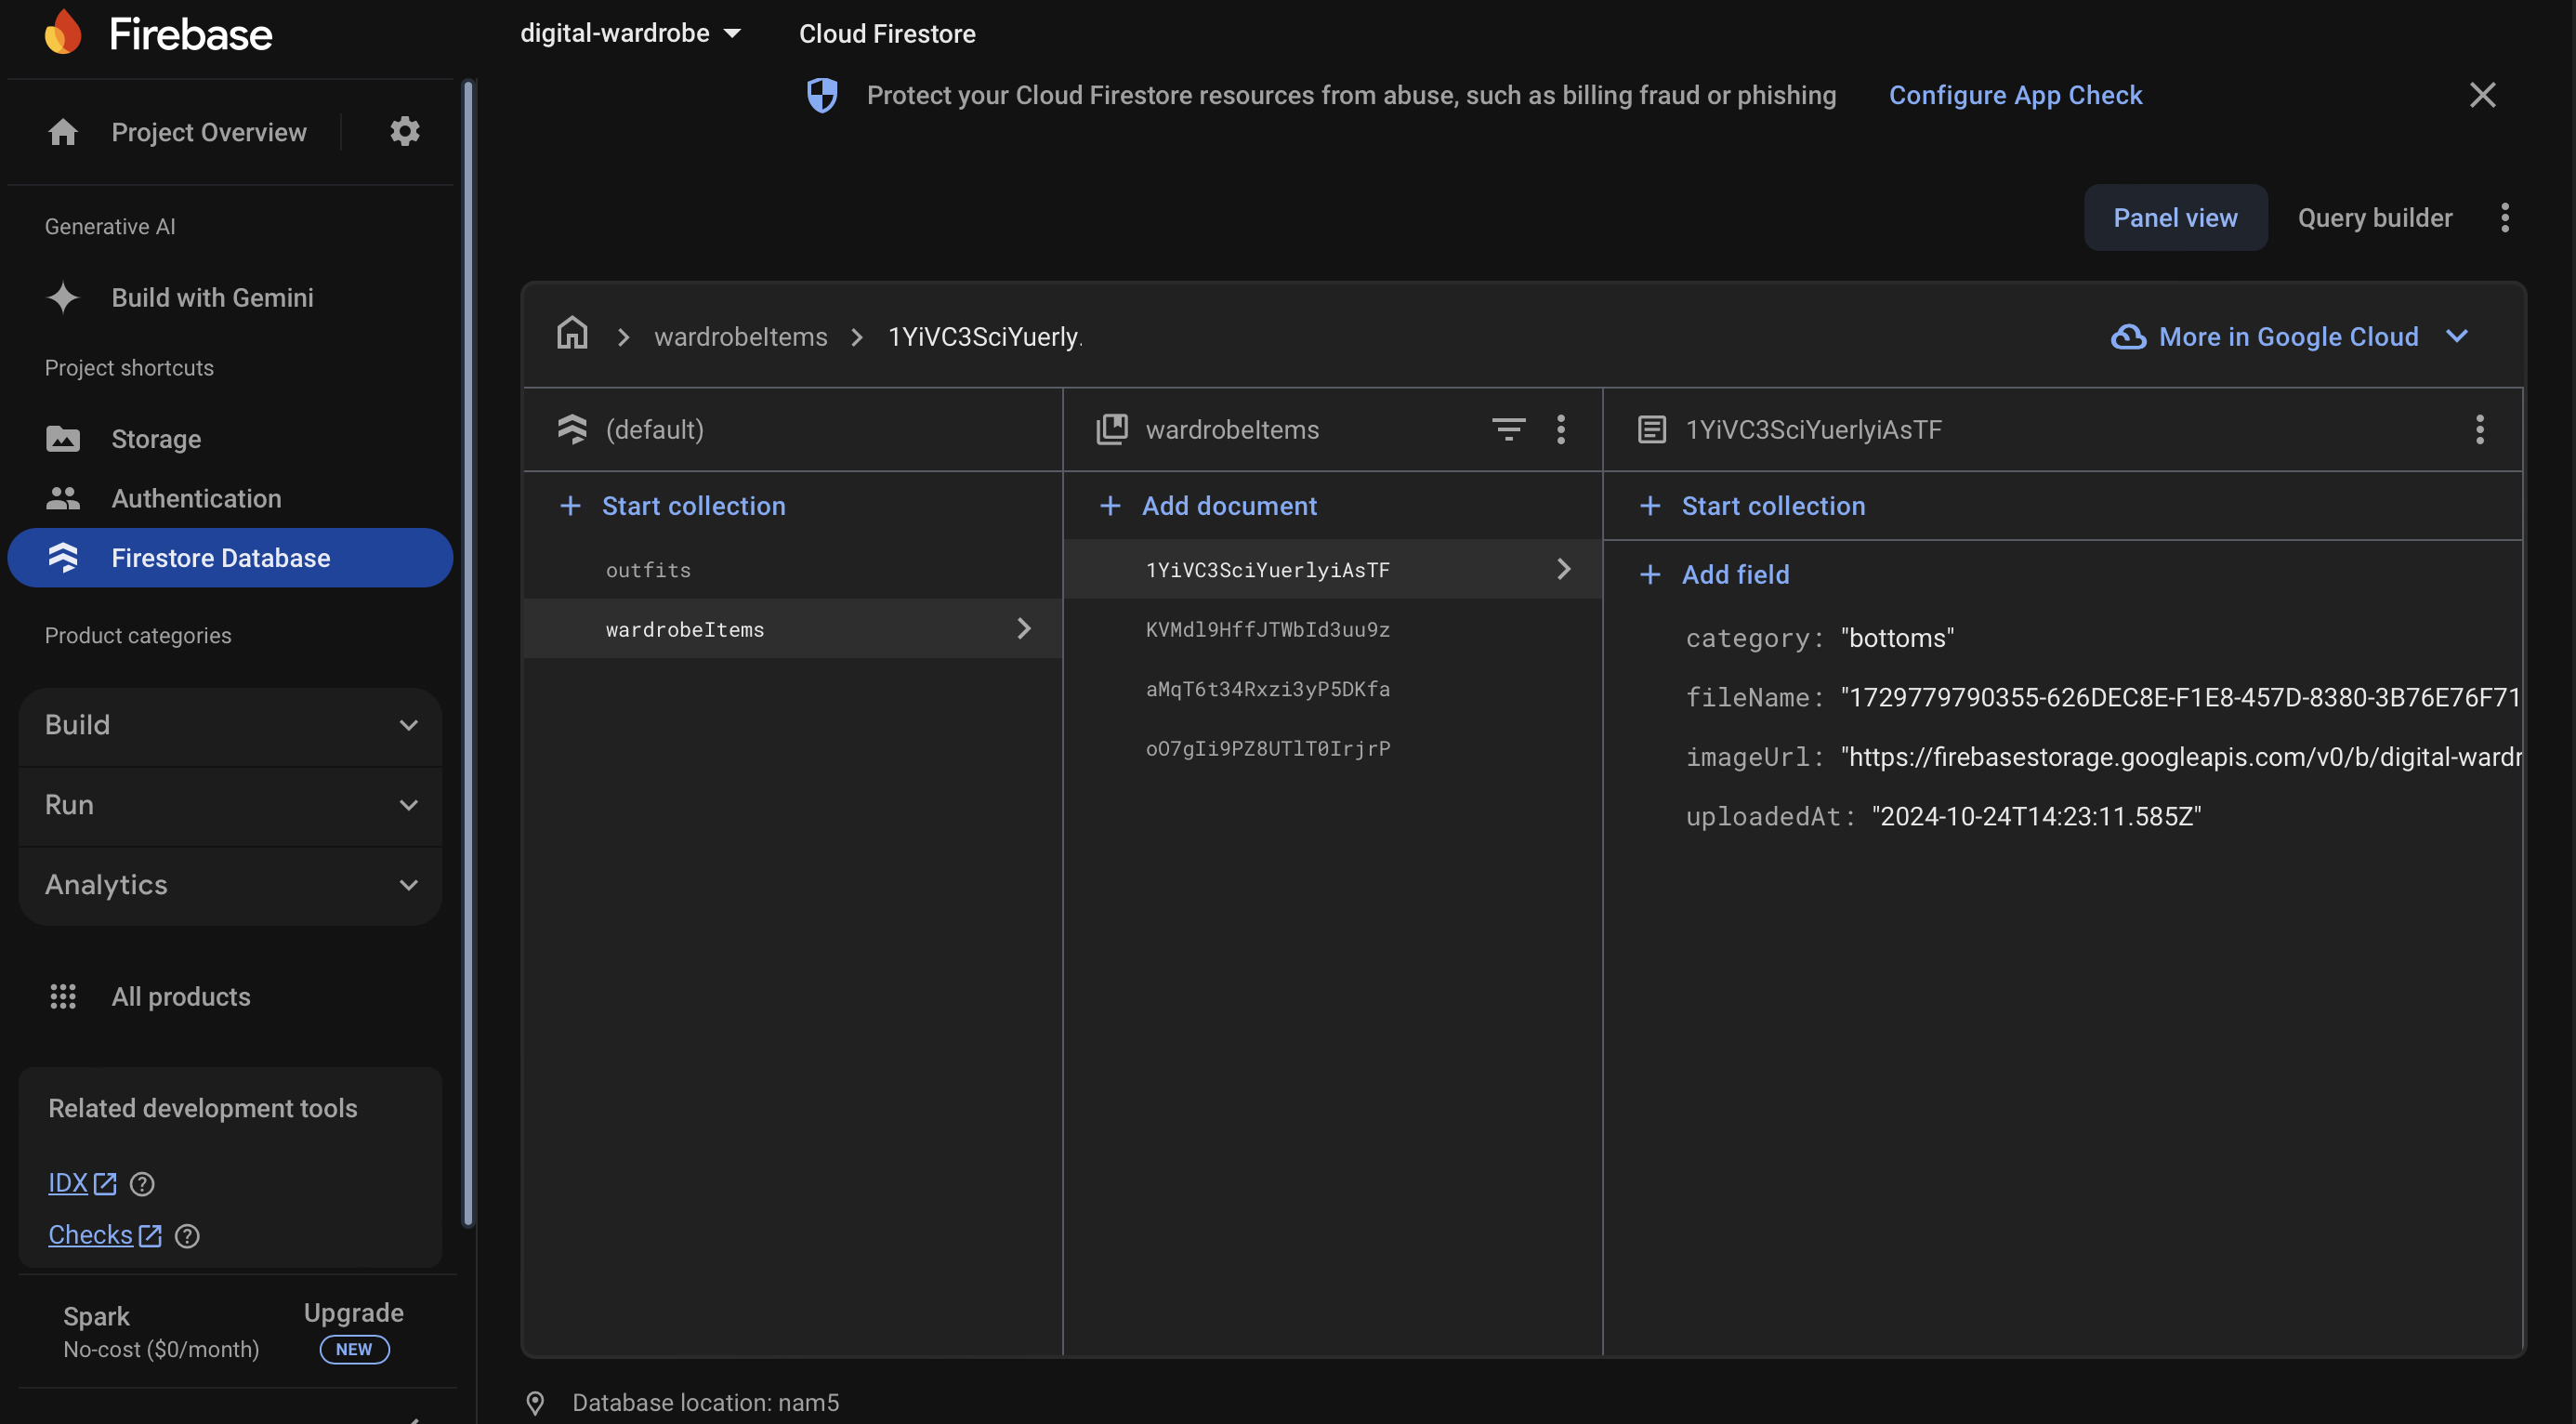
\includegraphics[width=0.8\textwidth]{exampleis-master/figures/wardrobeitemFB.png}\label{fig:wardrobe_items}}
    \qquad % Adds horizontal spacing between the images
    % Second Subfloat: Outfit Items
    \subfloat[Firestore structure for outfit combinations.][Outfit Items]
    {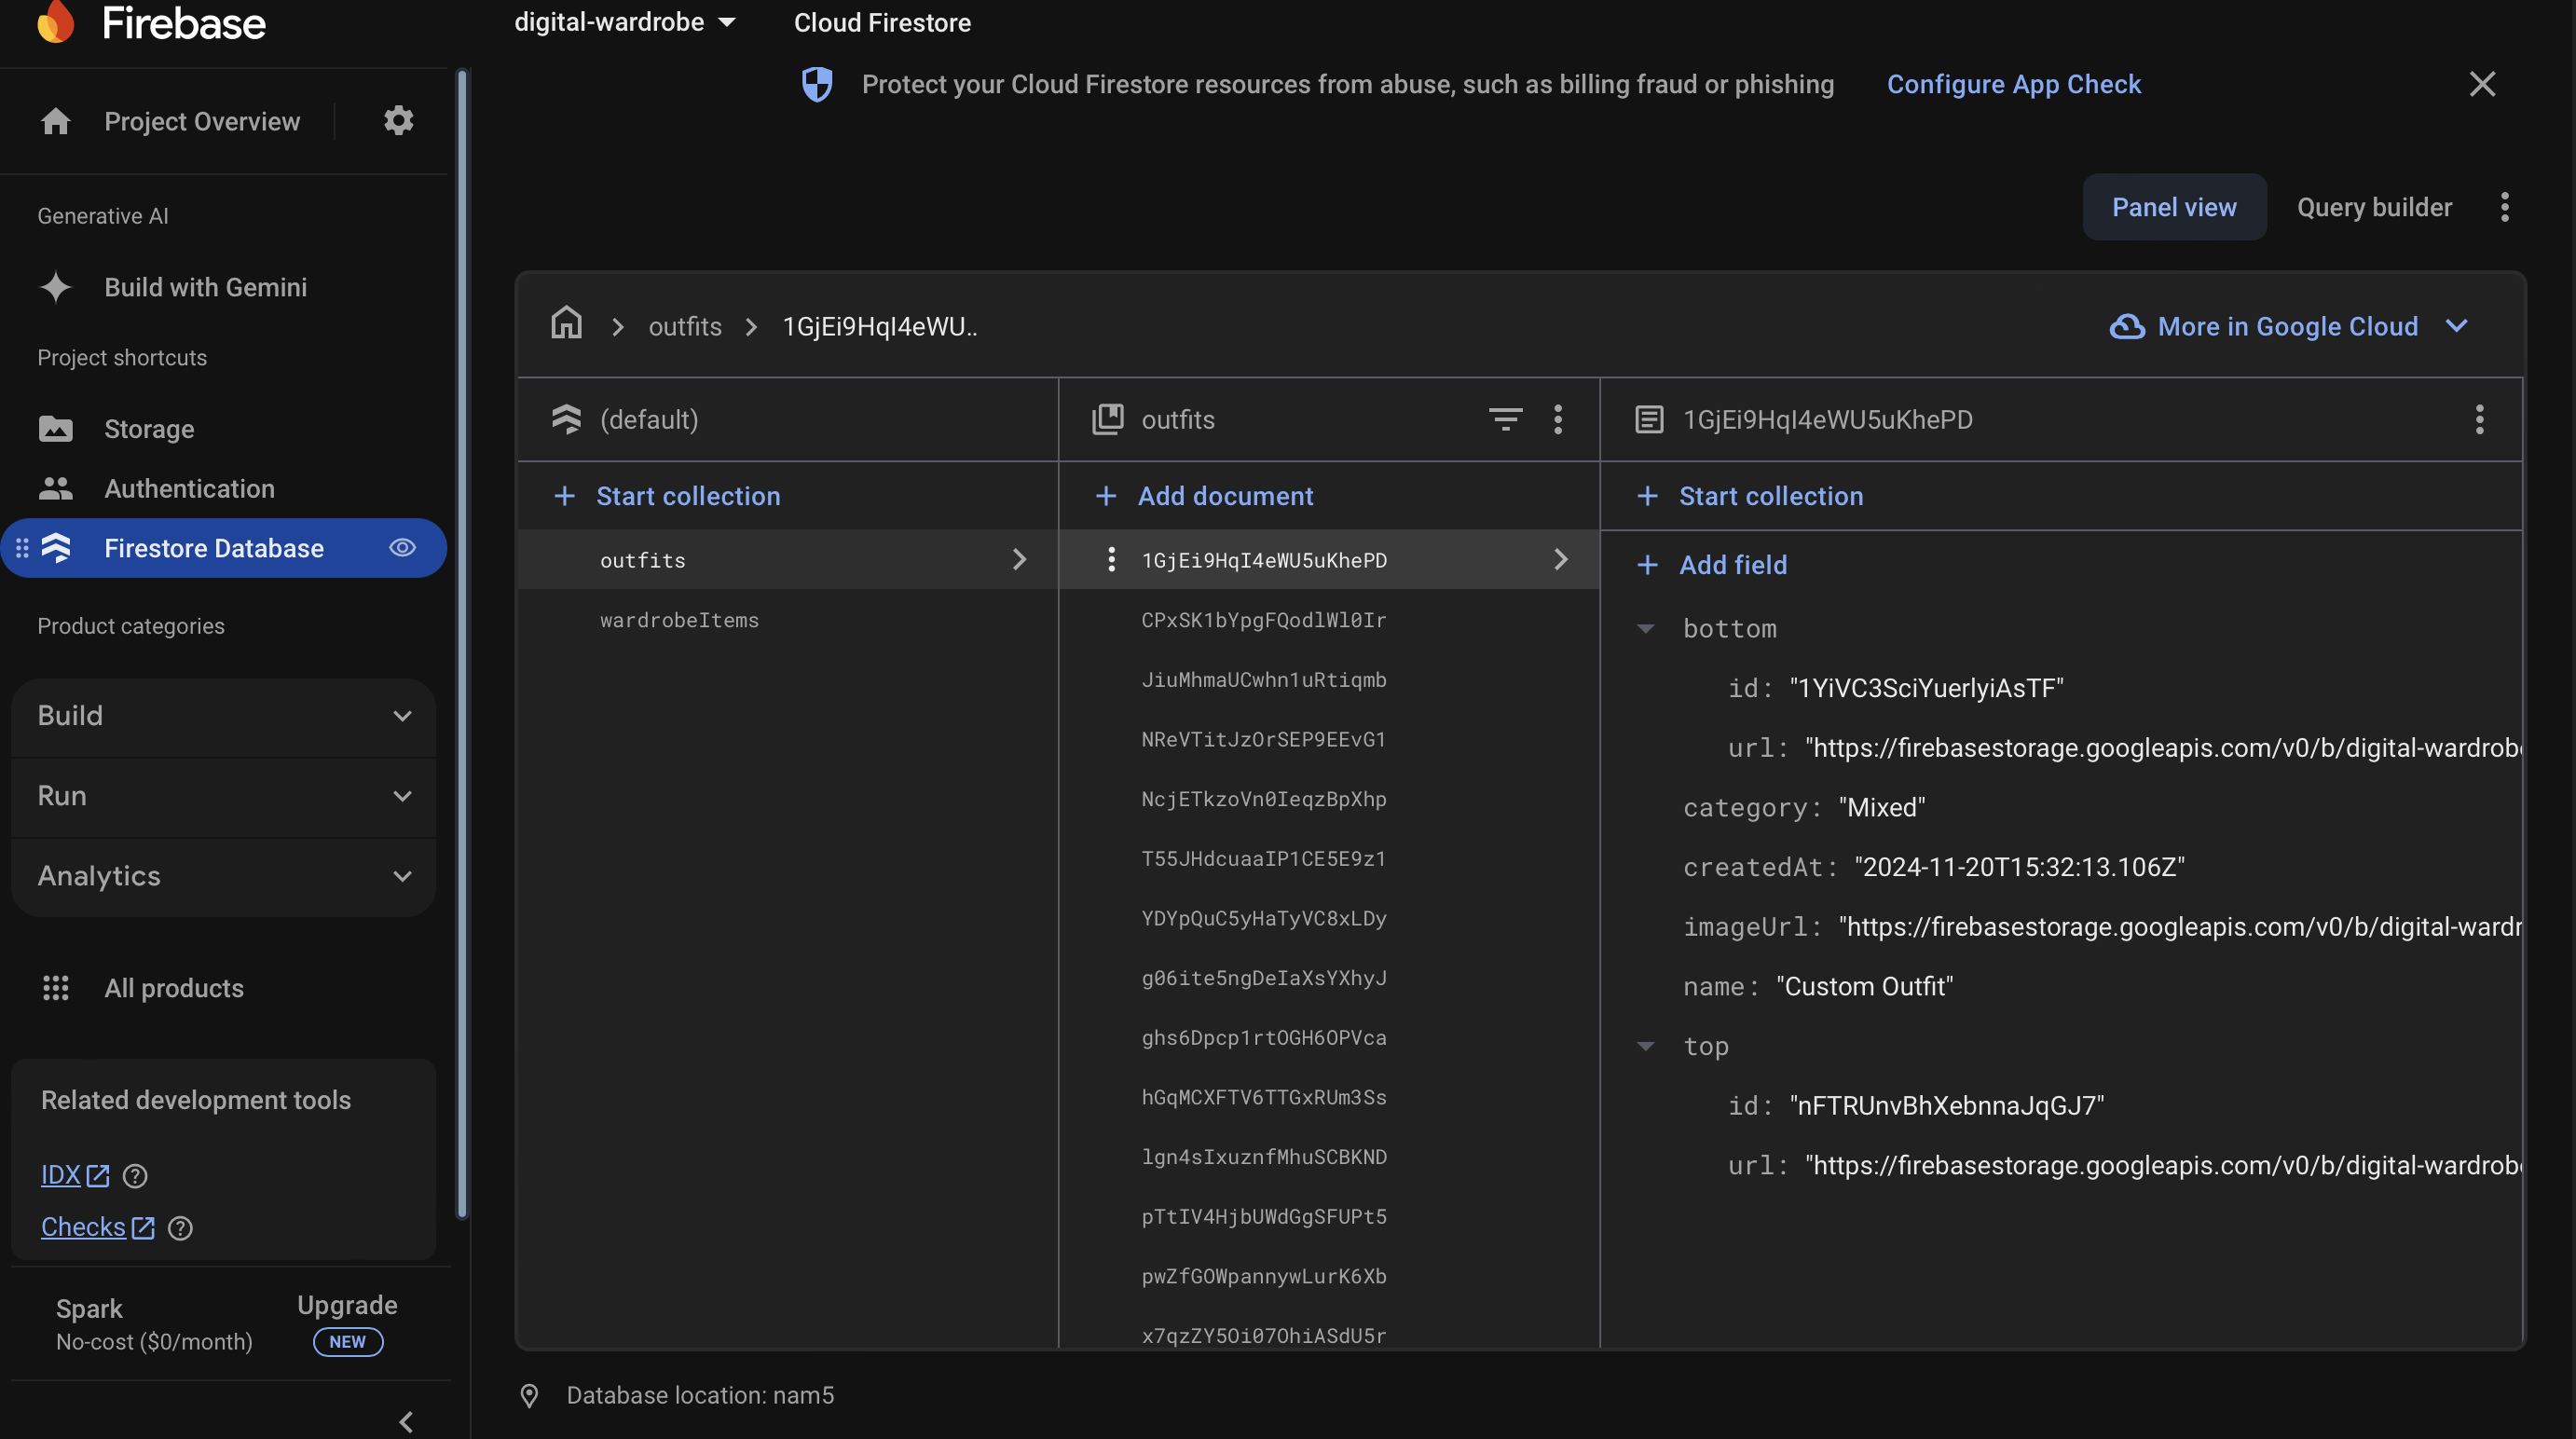
\includegraphics[width=0.8\textwidth]{exampleis-master/figures/OutfititemFB.png}\label{fig:outfit_items}}
    \caption{Firestore collections for wardrobe items and outfits.}
    \label{fig:firestore_collections}
\end{figure}


The integration of Firebase Cloud Storage and Firestore \textit{My Digital Wardrobe}provides a smooth and reliable experience, where users can easily organize and experiment with their wardrobe collections.

\section{Authentication and Security}

For \textit{My Digital Wardrobe}, ensuring that user data remains safe and accessible only to the right person is important. This is where authentication and security come into play. Think of authentication as the app's way of checking, "Who are you?" and security as the process of making sure that only the right people can see or change certain information.

Authentication in \textit{My Digital Wardrobe} is handled by \textbf{Firebase Authentication}, which allows users to sign in securely. Instead of building complicated login systems from scratch, Firebase provides easy-to-use tools for this purpose. Users can log in with an email and password or even through trusted services like Google or Facebook.

When a user logs in, Firebase creates a secure connection between the user and their personal wardrobe data. This ensures that only that user can view or edit their clothing items and outfits. It’s similar to how online banking systems require customers to log in before showing their account details—only they have access.


While authentication checks who they are, security rules decide what they can do. In My Digital Wardrobe, Firebase uses Firestore Security Rules to protect data. These rules ensure that each user can only see or change their wardrobe items, preventing unauthorized access.

For example, if two users use the app, User A cannot see or edit User B’s wardrobe. Firebase automatically checks who is making the request and allows or blocks access based on the security rules set for the app. This protects sensitive data and ensures privacy.

In Listing \ref{lst:firestore_rules} Firestore Security Rules enforce access policies for the database.

\begin{lstlisting}[caption={Firestore Security Rules}, label={lst:firestore_rules}]
rules_version = '2';
service cloud.firestore {
  match /databases/{database}/documents {
    match /{document=**} {
      allow read, write: if request.auth != null;
    }
  }
}
\end{lstlisting}

\noindent \textbf{Explanation of the Rules}:
\begin{itemize}
    \item \textbf{\texttt{rules\_version = '2'}}: Specifies the version of Firestore security rules being used.
    \item \textbf{\texttt{service cloud.firestore}}: Indicates the rules apply to Firestore, Firebase's NoSQL database service.
    \item \textbf{\texttt{match /databases/\{database\}/documents}}: Defines the scope of the rules, targeting all documents within the database.
    \item \textbf{\texttt{match /{document=**}}}: Includes all document paths, including nested sub-collections.
    \item \textbf{\texttt{allow read, write: if request.auth != null}}: Grants read and write permissions only to authenticated users (\texttt{request.auth != null} ensures that the request is made by a logged-in user).
\end{itemize}
In simple terms, this means that unless the user has been authenticated (logged in), they cannot access any data. These rules apply to all parts of the wardrobe, ensuring that no unauthorized person can view or change the information.

Beyond controlling who can access the data, My Digital Wardrobe uses encryption to protect information when it’s being transferred between the app and Firebase’s servers. Think of encryption as converting the data into a secret code while it’s moving, so no one can read it if they intercept it. Once the data reaches its destination, it is decoded back to its original form. This ensures that even when users upload images or log in from different networks, their data remains secure and protected from potential threats.

Without proper authentication and security measures, anyone could access, modify, or delete user data. For an app like My Digital Wardrobe, this could mean losing carefully organized wardrobe collections or exposing personal images to others. By using Firebase's authentication and security tools, the app ensures that:
\begin{itemize}
    \item Each user’s data remains private.
    \item Unauthorized users cannot gain access.
    \item All communication between the app and the backend is protected.
\end{itemize}
The combination of Firebase Authentication and Firestore Security Rules forms a strong system that builds trust and ensure that users can confidently manage their wardrobes, knowing that their data is secure.

With a robust architecture in place, the next chapter will explore how these technologies and systems were brought to life through practical development. It will detail the step-by-step process of building the app’s key features, from user interface design and navigation flows to image uploading and outfit creation. The chapter will also discuss design principles that guided the creation of an intuitive user experience.